% !TEX root = ../presentation.tex
% !BIB program = biber
% !TEX program = xelatex

\section{a brief overview of unsupervised speech representation learning}


\begin{frame}
    \frametitle{Overview: Representation Learning for Speech}

    \begin{columns}

        \begin{column}{0.4\textwidth}
            \begin{itemize}
                \item We focus on two primary categories:
                \begin{itemize}
                    \item Self-supervised learning (SSL)
                    \item Probabilistic latent variable models (LVMs)
                \end{itemize}
                \item Recent developments have been driven by self-supervised learning.
                \item A model-by-model overview: Focus on speech recognition.
            \end{itemize}
        \end{column}

        \begin{column}{0.6\textwidth}

            \begin{tikzpicture}
                \only<1->{
                    \node[anchor=south west,inner sep=0] (A) at (0,0) {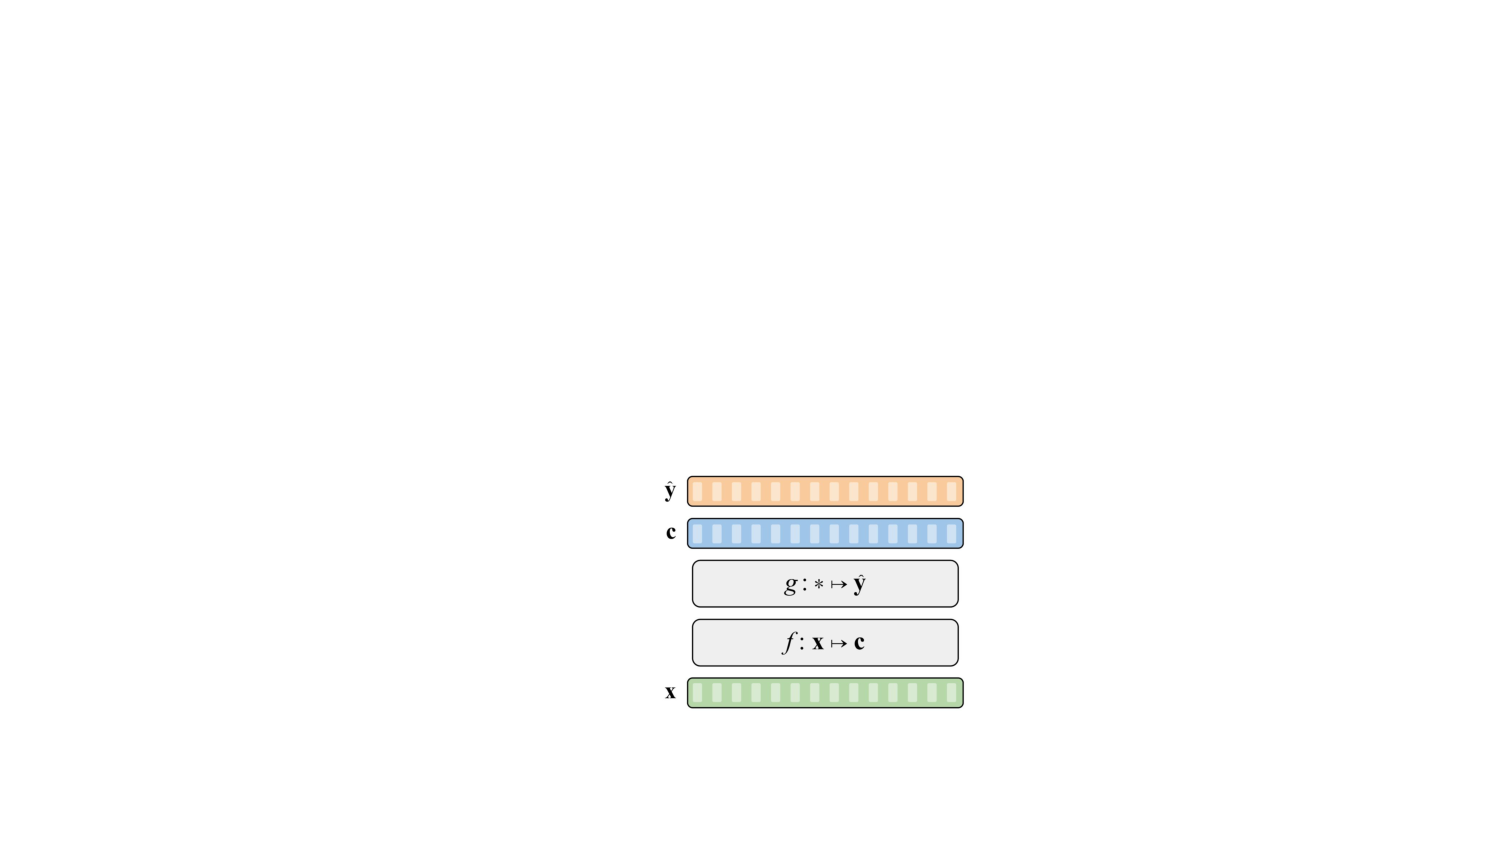
\includegraphics[height=0.4\textheight]{figures/brief-paradigms-ssl.pdf}};
                    \node[anchor=south west,inner sep=0] (B) at (4.2,0) {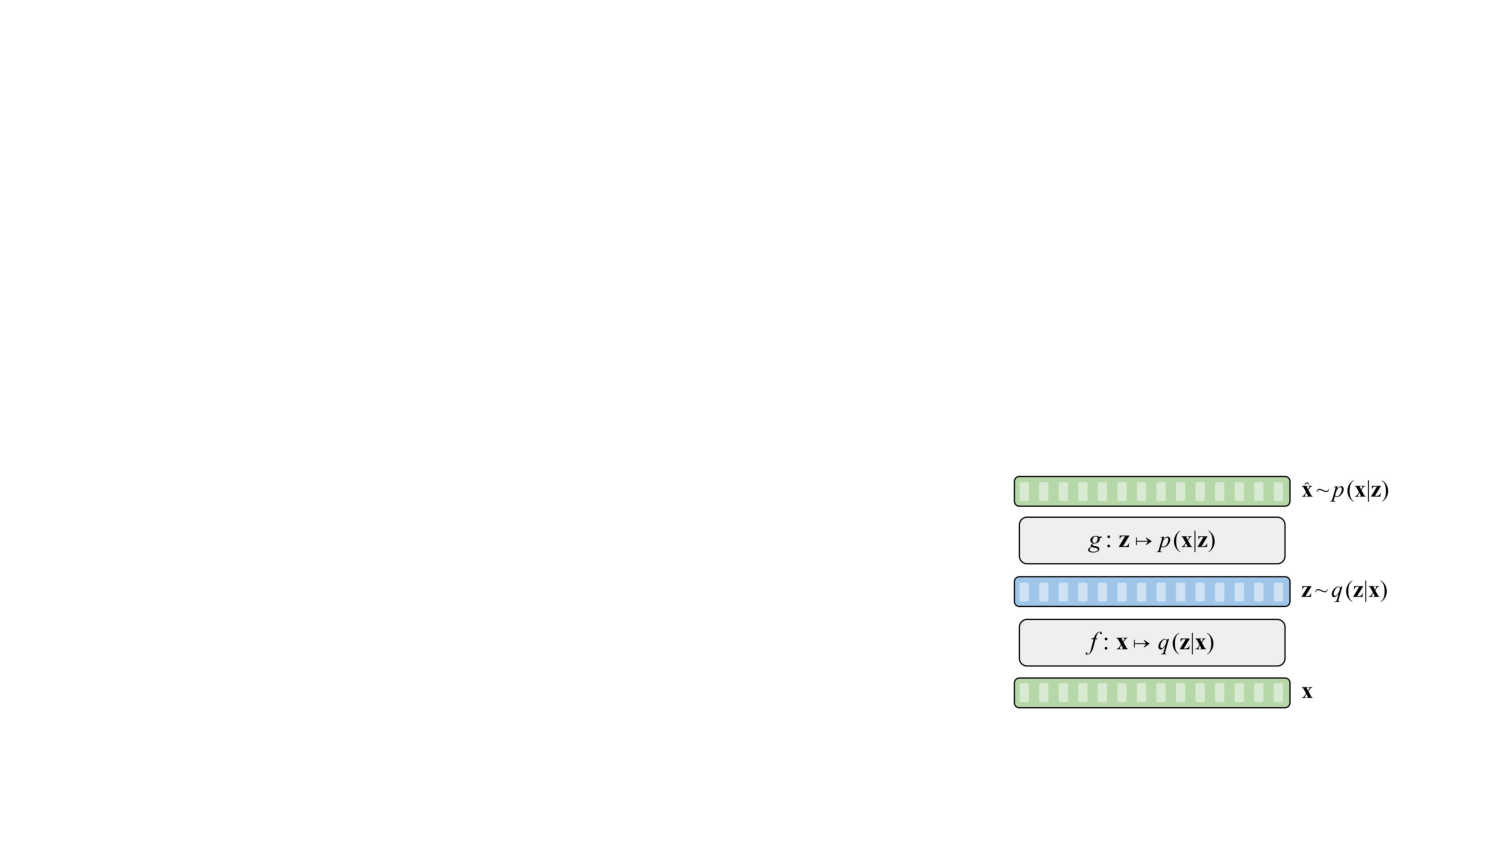
\includegraphics[height=0.4\textheight]{figures/brief-paradigms-lvm-2.pdf}};
                }
            
                \only<2->{
                    \node[anchor=south west,inner sep=0] (A) at (0,0) {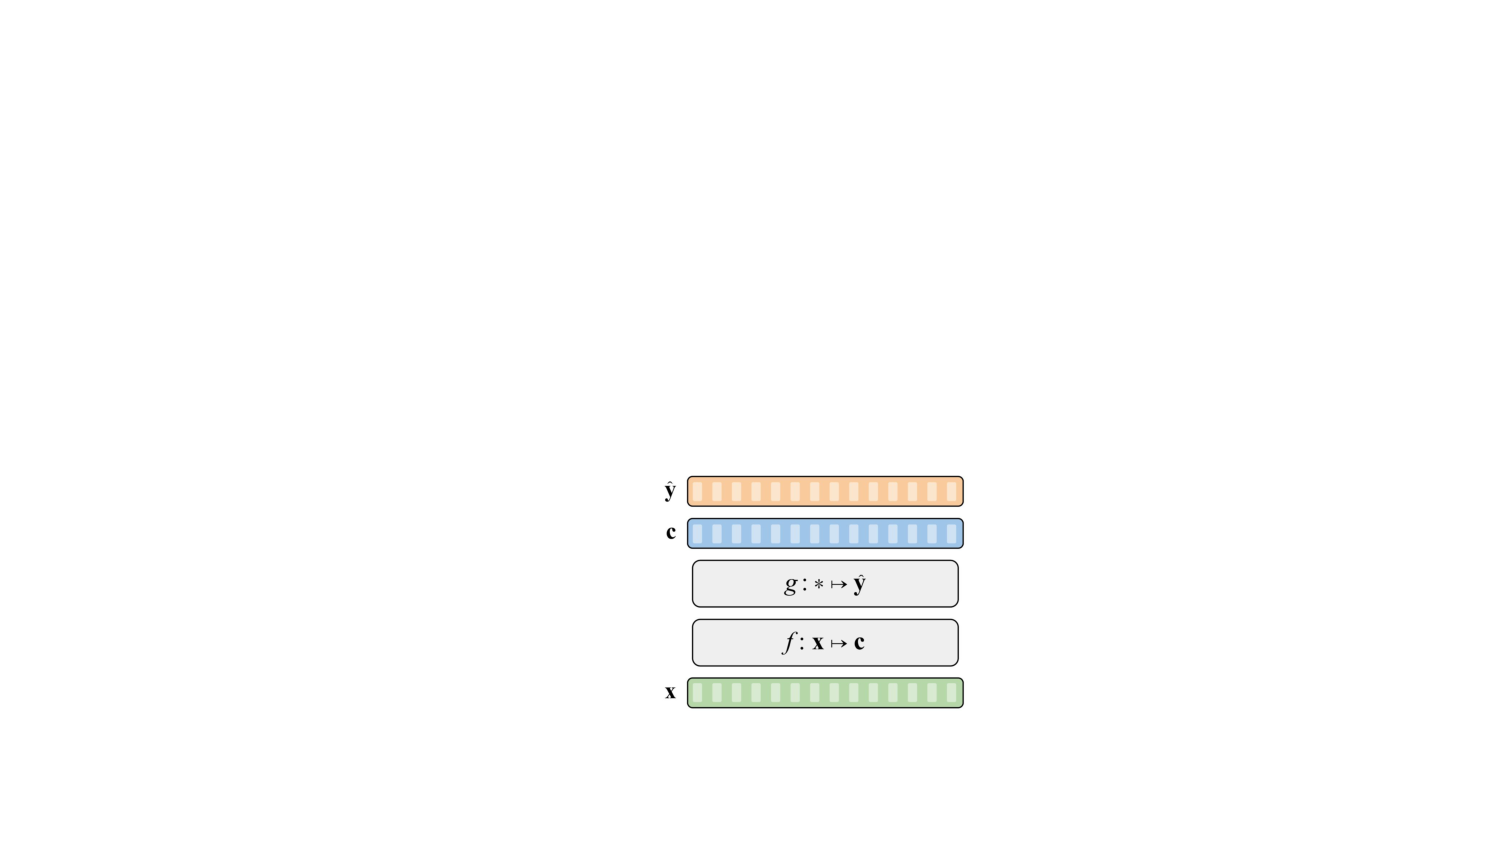
\includegraphics[height=0.4\textheight]{figures/brief-paradigms-ssl.pdf}};
                    \node[anchor=south west,inner sep=0] (B) at (4.2,0) {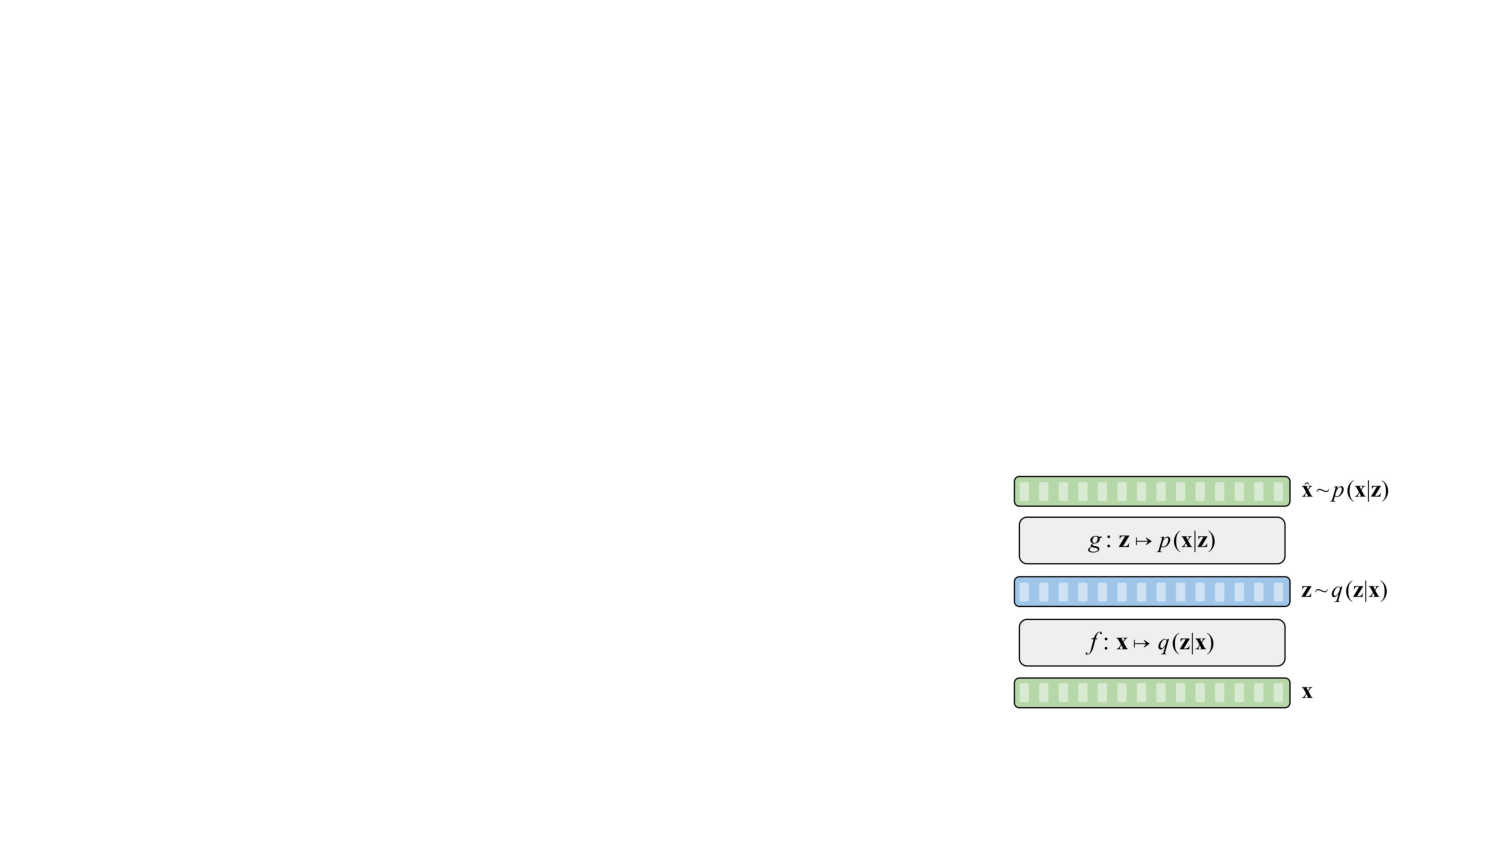
\includegraphics[height=0.4\textheight]{figures/brief-paradigms-lvm-2.pdf}};
                    \fill [draw=none, fill=white, fill opacity=0.7] (B.north west) -- (B.north east) -- (B.south east) -- (B.south west) -- (B.north west) -- cycle;
                }
            \end{tikzpicture}

        \end{column}
        
    \end{columns}
\end{frame}


\begin{frame}
    \frametitle{\vphantom{ABCDEFGHJIJKLMNOPQRSTVWXYZ}{Development of SSL for speech}}
    \begin{columns}[t]
        \hspace{0.025\textwidth}
        \begin{column}{0.20\textwidth}
            \begin{figure}[\textwidth]
                \centering
                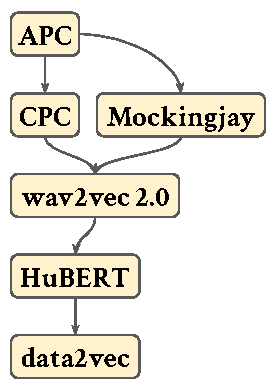
\includegraphics[width=\textwidth]{figures/brief-flow-0.pdf}
            \end{figure}
        \end{column}
        {\textcolor{black!40}{\vrule{}}}
        \begin{column}{0.40\textwidth}
            {\vspace{0.10\textheight}\footnotesize}
        \end{column}
        \begin{column}{0.30\textwidth}
            \begin{figure}[2.333\textwidth]
                % \centering
                % 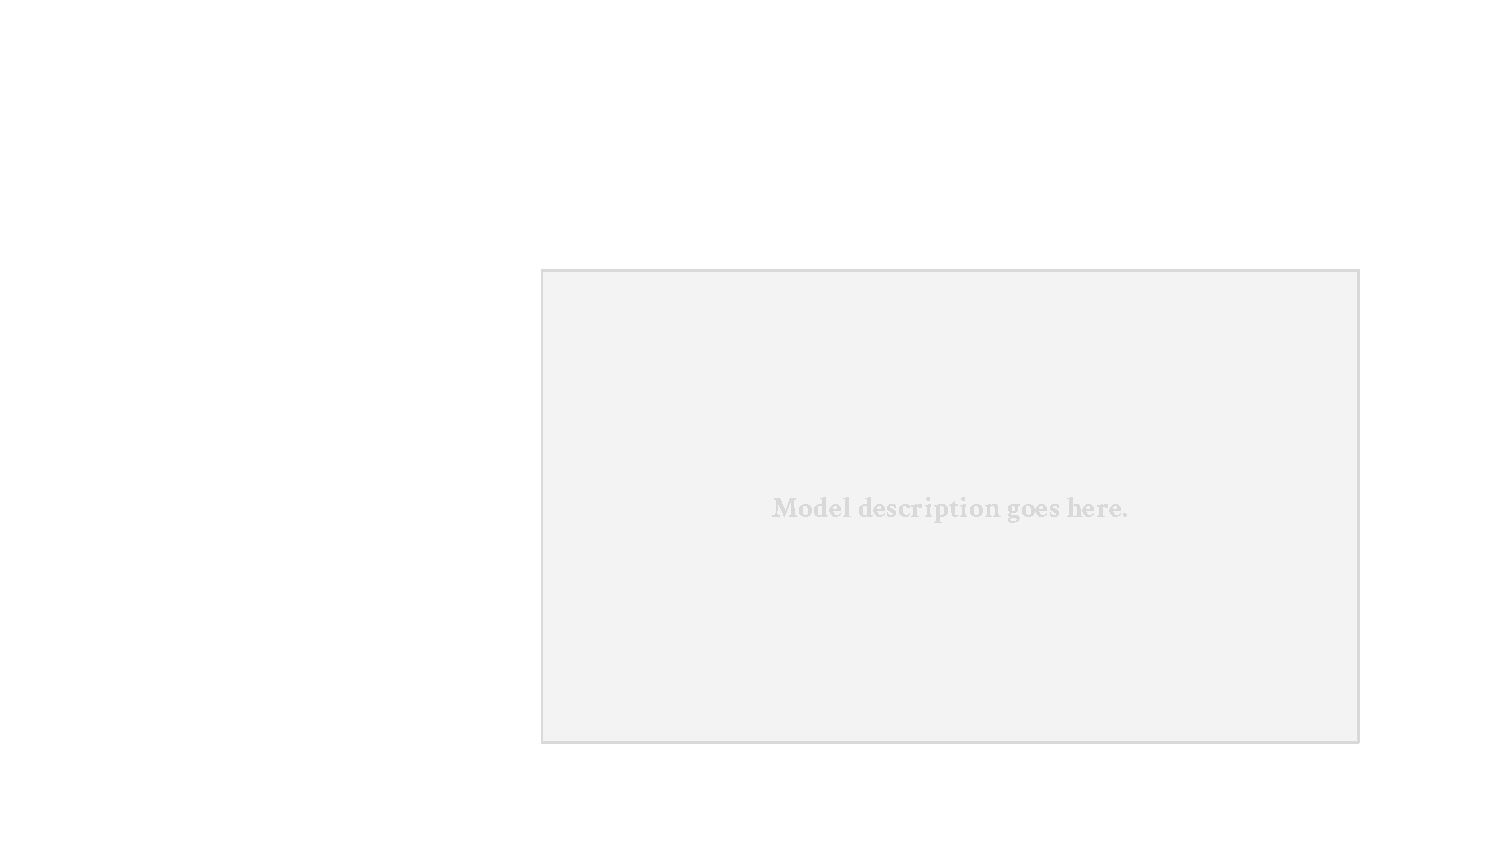
\includegraphics[width=2.333\textwidth]{figures/brief-model-0.pdf}
            \end{figure}
        \end{column}
        % \hspace{0.020\textwidth}
        % \begin{column}{0.70\textwidth}
        %     \centering
        %     \begin{figure}[\textwidth]
        %         \centering
        %         {\vspace{0.2\textheight}\color{black!40}\scshape model description goes here}
        %     \end{figure}
        % \end{column}
        \hspace{0.020\textwidth}
    \end{columns}
\end{frame}


{ % start font size change group

\setbeamerfont*{itemize/enumerate body}{size=\fontsize{8}{10}}
\setbeamerfont*{itemize/enumerate subbody}{parent=itemize/enumerate body}
\setbeamerfont*{itemize/enumerate subsubbody}{parent=itemize/enumerate body}

\newcommand{\presentationbriefslide}[3]{%
    \begin{frame}
        \frametitle{\vphantom{ABCDEFGHJIJKLMNOPQRSTVWXYZ}{#2}}
        \begin{columns}[t]
            \hspace{0.025\textwidth}
            \begin{column}{0.20\textwidth}
                \begin{figure}[\textwidth]
                    \centering
                    \includegraphics[width=\textwidth]{figures/brief-flow-#1.pdf}
                \end{figure}
            \end{column}
            {\textcolor{black!40}{\vrule{}}}
            \begin{column}{0.40\textwidth}
                {\vspace{0.10\textheight}\footnotesize#3}
            \end{column}
            \begin{column}{0.30\textwidth}
                \begin{figure}[\textwidth]
                    \centering
                    \includegraphics[width=\textwidth]{figures/brief-model-#1.pdf}
                \end{figure}
            \end{column}
            \hspace{0.020\textwidth}
        \end{columns}
    \end{frame}
}

% \presentationbriefslide{0}{Development of SSL for speech}{}%

\presentationbriefslide{1}{Autoregressive Predictive Coding (APC)}{%
    \begin{itemize}
        \item {\bfseries \color{black} Task}: Predict future inputs.
        \item {\bfseries \color{black} Input/target}: Log-mel spectrogram.
        \item {\bfseries \color{black} Architecture}: RNN/Transformer decoder.
        \item {\bfseries \color{black} Slow features}: Predict $k$ steps ahead.
    \end{itemize}
}

\presentationbriefslide{2}{Autoregressive Predictive Coding (APC)}{%
    \begin{itemize}
        \item {\bfseries \color{black} Challenges}:
        \begin{itemize}
            \item Encodes only past inputs \xmark
            \item Uses the input as target \xmark
        \end{itemize}
    \end{itemize}
}

\presentationbriefslide{3}{Mockingjay}{%
    \begin{itemize}
        \item {\bfseries \color{black} Task}: Reconstruct masked inputs.
        \item {\bfseries \color{black} Architecture}: Transformer encoder.
        \item {\bfseries \color{black} Masking}: 
        \begin{itemize}
            \item $X$\% at random. (Mockingjay)
            \item $X$\% + $N$ consecutive (wav2vec 2.0)
            \item SpecAugment (Masked RNN)
        \end{itemize}
    \end{itemize}
}

\presentationbriefslide{4}{Mockingjay}{%
    \begin{itemize}
        \item {\bfseries \color{black} Challenges}:
        \begin{itemize}
            \item Encodes the entire input \cmark
            \item Uses the input as target \xmark
        \end{itemize}
    \end{itemize}
}

\presentationbriefslide{5}{Contrastive Predictive Coding (CPC)}{%
    \begin{itemize}
        \item {\bfseries \color{black} Contrastive models}: Distinguish target samples from negative samples.
        \item {\bfseries \color{black} Learned target}: Discard details.
        \item {\bfseries \color{black} Sampling negatives}:
        \begin{itemize}
            \item Sample sequence?
            \item Same speaker?
        \end{itemize}
    \end{itemize}
}

\presentationbriefslide{6}{Contrastive Predictive Coding (CPC)}{%
    \begin{itemize}
        \item {\bfseries \color{black} Challenges}:
        \begin{itemize}
            \item <1-> Only encodes past inputs \xmark
            \item <1-> Uses a learned target \cmark
            \item <2-> Sampling negatives \xmark
        \end{itemize}
    \end{itemize}
}

\presentationbriefslide{8}{wav2vec 2.0} WER.
            \item 10 mimutes: \textbf{4.8\%} WER.
        \end{itemize}
    \end{itemize}
}

\presentationbriefslide{9}{wav2vec 2.0}{%
    \begin{itemize}
        \item {\bfseries \color{black} Challenges}:
        \begin{itemize}
            \item Encodes the entire input \cmark
            \item Uses a learned target \cmark
            \item Sampling negatives \xmarkshaded
        \end{itemize}
    \end{itemize}
}

\presentationbriefslide{10}{Hidden-unit BERT (HuBERT)}{%
    \begin{itemize}
        \item {\bfseries \color{black} Target}: $K$-means teacher.
        \item {\bfseries \color{black} Training}: Simple cross-entropy loss.
        \item {\bfseries \color{black} 1st iteration}: $K$-means on inputs.
    \end{itemize}
}


\presentationbriefslide{11}{Hidden-unit BERT (HuBERT)}{%
    \begin{itemize}
        \item {\bfseries \color{black} Target}: $K$-means teacher.
        \item {\bfseries \color{black} Training}: Simple cross-entropy loss.
        \item {\bfseries \color{black} 1st iteration}: $K$-means on inputs.
        \item {\bfseries \color{black} 2nd iteration}: $K$-means on hidden layers.
    \end{itemize}
}


\presentationbriefslide{12}{Hidden-unit BERT (HuBERT)}{%
    \begin{itemize}
        \item {\bfseries \color{black} Challenges}:
        \begin{itemize}
            \item <1-> Encodes the entire input \cmark
            \item <1-> Uses a learned target \cmark
            \item <1-> No need for negative samples \cmark
            \item <2-> Targets updated infrequently \xmark
            \item <2-> Quantized targets \xmark
        \end{itemize}
    \end{itemize}
}

\presentationbriefslide{14}{data2vec}{%
    \begin{itemize}
        \item Uses a teacher-student framework.
        \item {\bfseries \color{black} Teacher}:
        \begin{itemize}
            \item EMA of student (online) \cmark
            \item Target is average of top $K$ layers \cmark
        \end{itemize}
    \end{itemize}
}

\presentationbriefslide{15}{data2vec}{%
    \begin{itemize}
        \item Uses a teacher-student framework.
        \item {\bfseries \color{black} Teacher}:
        \begin{itemize}
            \item EMA of student (online) \cmark
            \item Target is average of top $K$ layers \cmark
        \end{itemize}
        \item {\bfseries \color{black} Student training}: Smooth $\l_1$ loss.
    \end{itemize}
}

\presentationbriefslide{16}{data2vec}{%
    \begin{itemize}
        \item {\bfseries \color{black} Challenges}:
        \begin{itemize}
            \item Encodes the entire input \cmark
            \item Uses a learned target \cmark
            \item No need for negative samples \cmark
            \item Targets updated continuously \cmark
            \item Continuous-valued targets \cmark
        \end{itemize}
    \end{itemize}
}


} % end font size change group


\begin{frame}
    \frametitle{Overview: Representation Learning for Speech}

    \begin{columns}

        \begin{column}{0.4\textwidth}
            \begin{itemize}
                \item We focus on two primary categories:
                \begin{itemize}
                    \item Self-supervised learning (SSL)
                    \item Probabilistic latent variable models (LVMs)
                \end{itemize}
                \item Recent developments have been driven by self-supervised learning.
                \item A model-by-model overview: Focus on speech recognition.
            \end{itemize}
        \end{column}

        \begin{column}{0.6\textwidth}

            \begin{tikzpicture}
                \only<1->{
                    \node[anchor=south west,inner sep=0] (A) at (0,0) {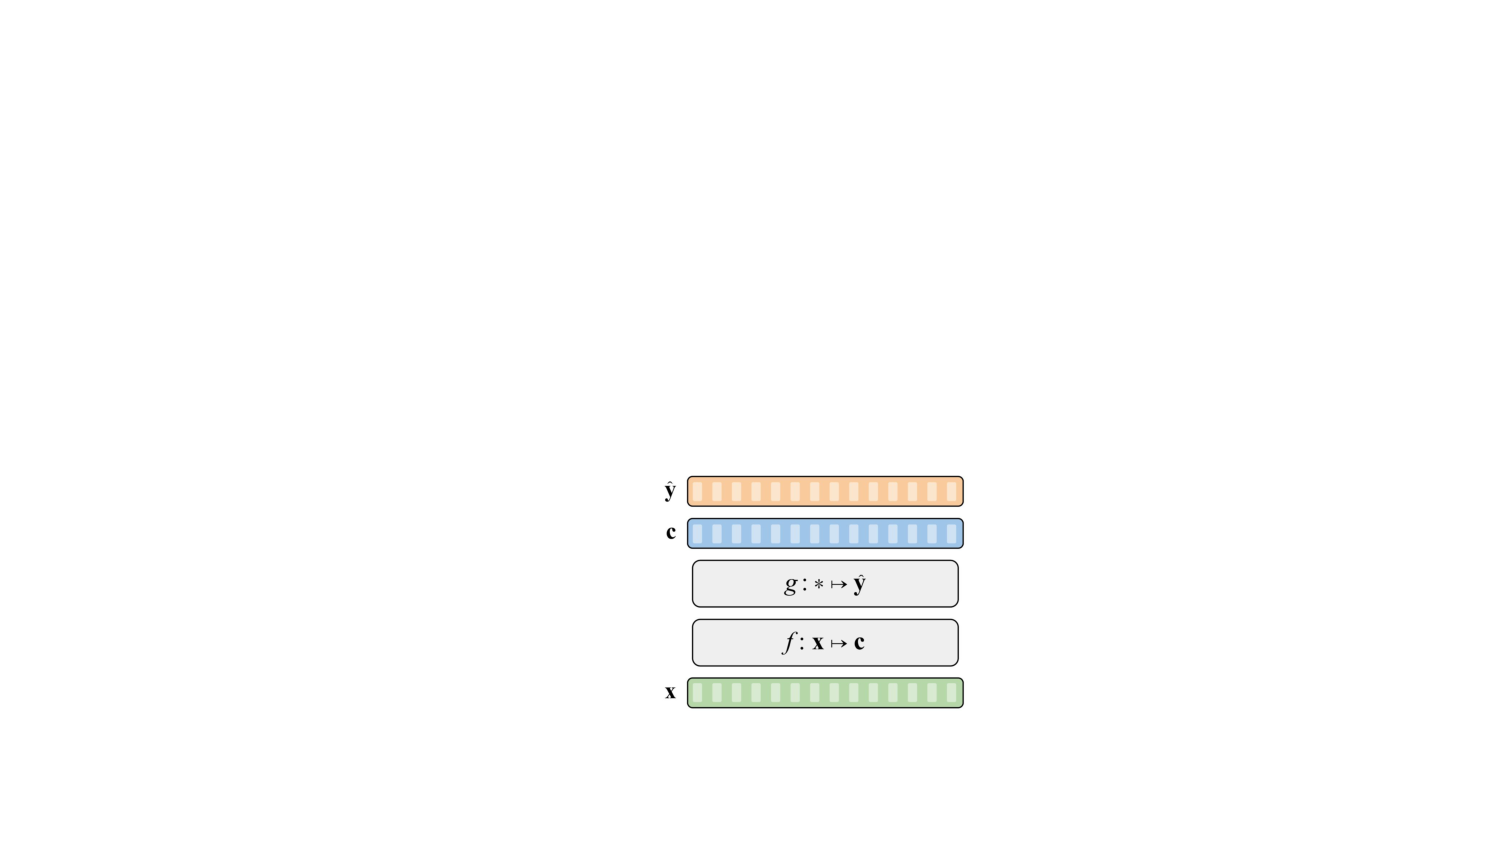
\includegraphics[height=0.4\textheight]{figures/brief-paradigms-ssl.pdf}};
                    \node[anchor=south west,inner sep=0] (B) at (4.2,0) {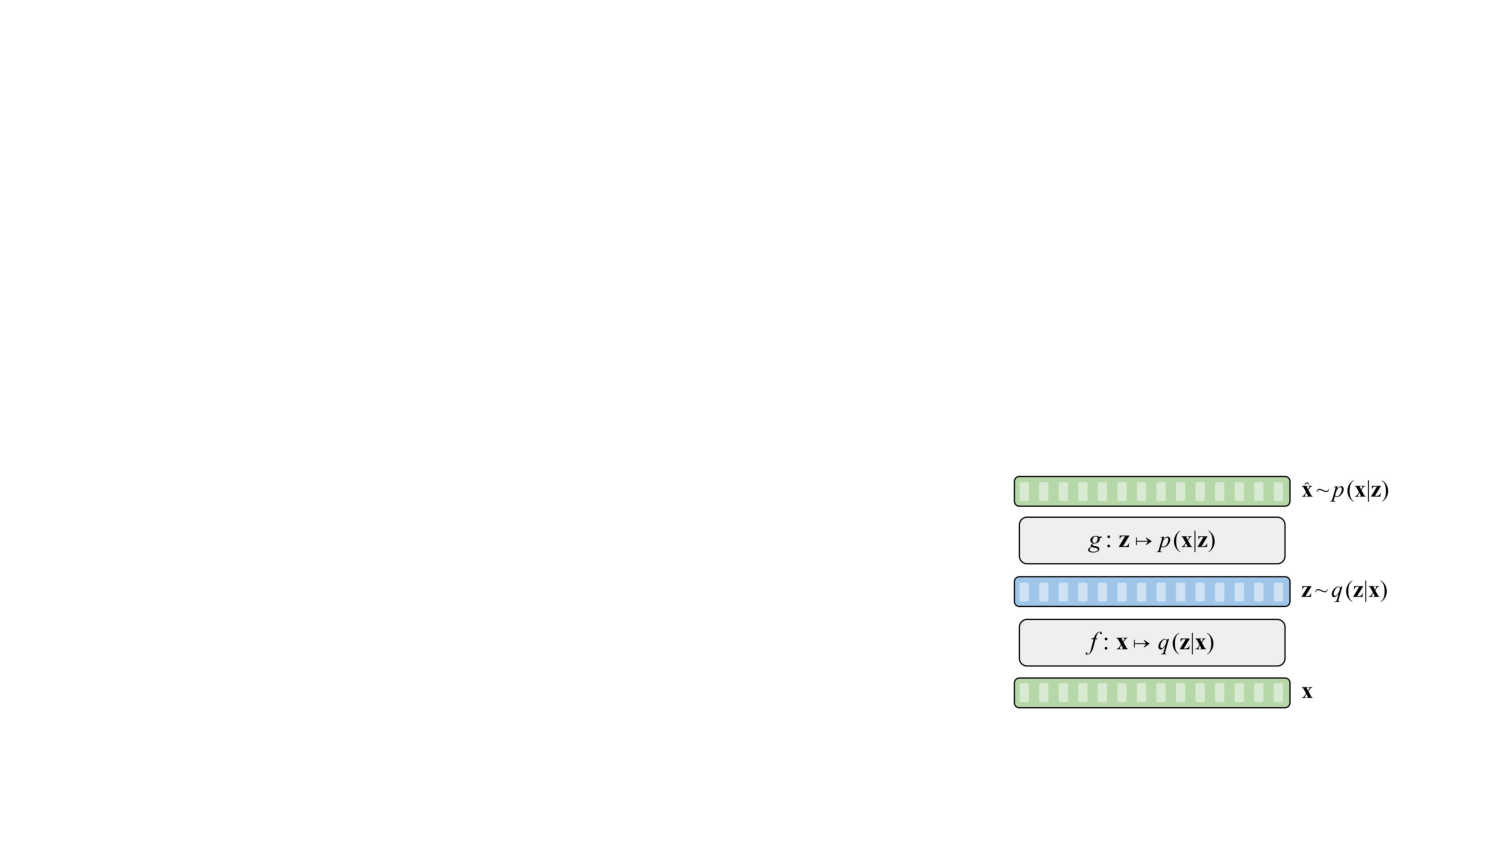
\includegraphics[height=0.4\textheight]{figures/brief-paradigms-lvm-2.pdf}};
                    \fill [draw=none, fill=white, fill opacity=0.7] (B.north west) -- (B.north east) -- (B.south east) -- (B.south west) -- (B.north west) -- cycle;
                }

                \only<2->{
                    \node[anchor=south west,inner sep=0] (A) at (0,0) {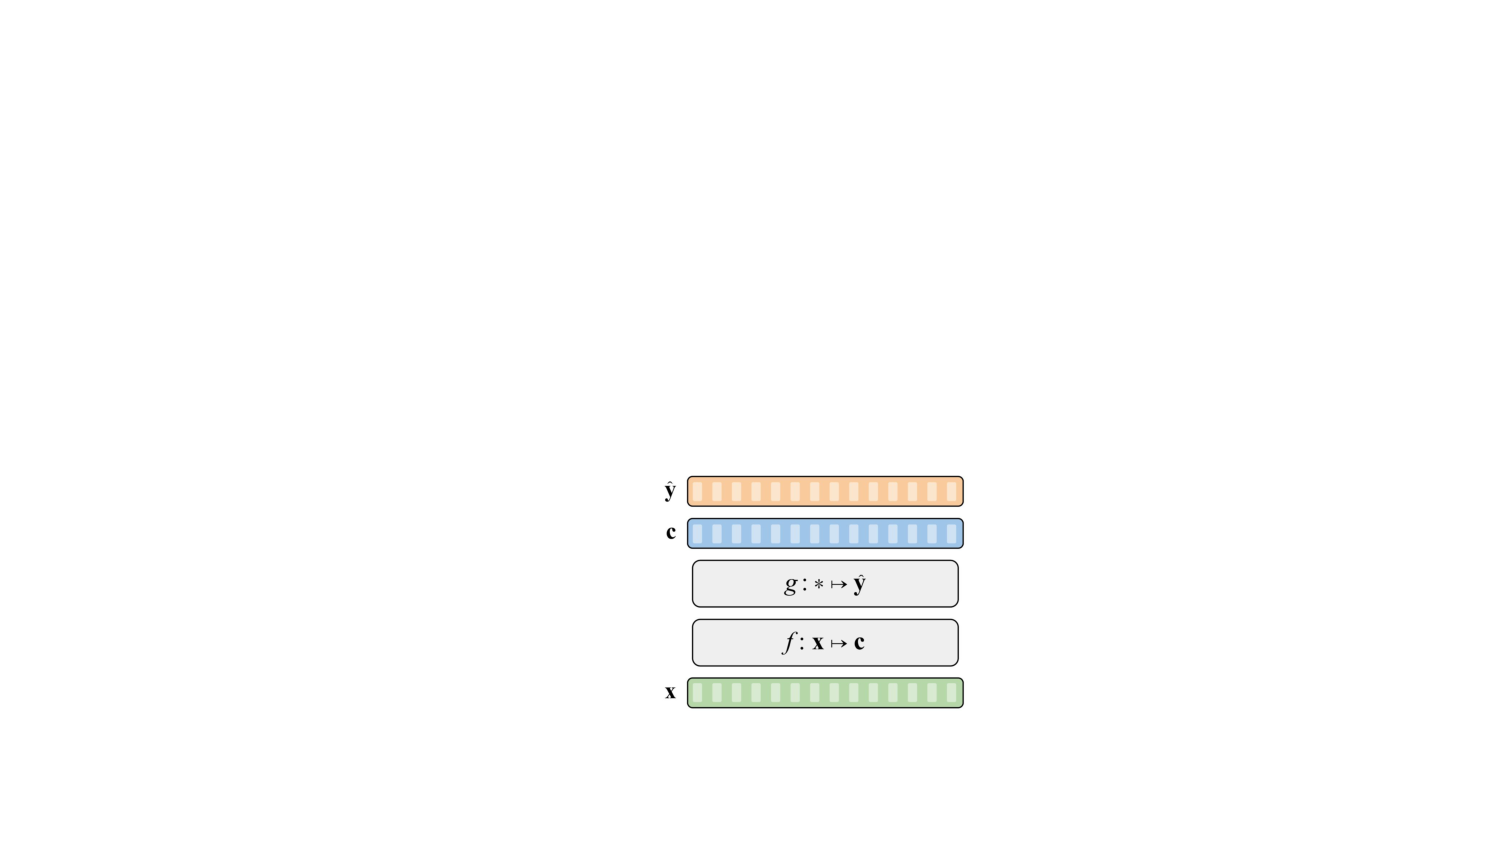
\includegraphics[height=0.4\textheight]{figures/brief-paradigms-ssl.pdf}};
                    \node[anchor=south west,inner sep=0] (B) at (4.2,0) {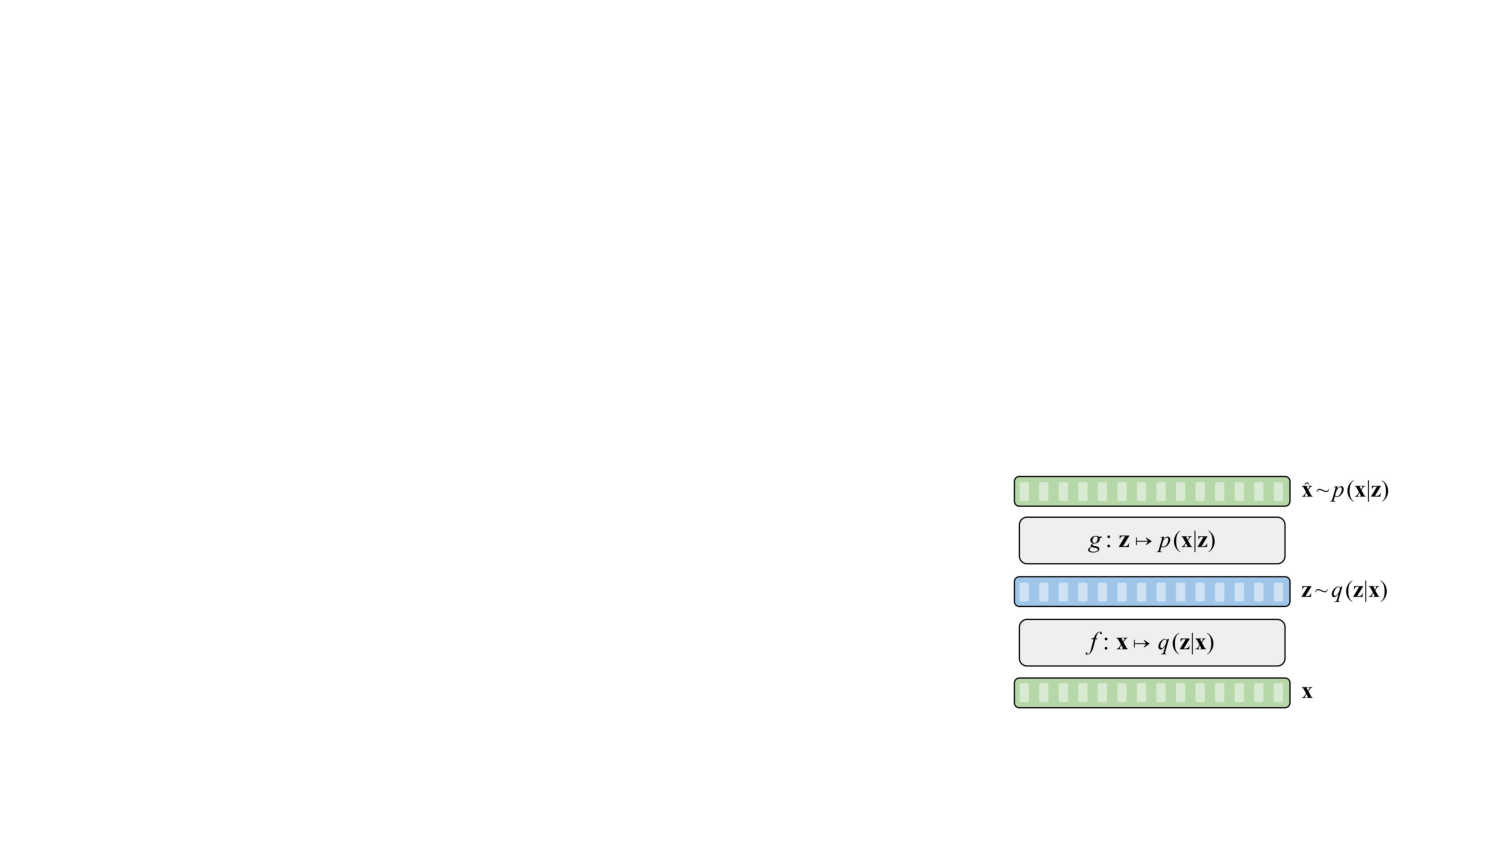
\includegraphics[height=0.4\textheight]{figures/brief-paradigms-lvm-2.pdf}};
                    \fill [draw=none, fill=white, fill opacity=0.7] (A.north west) -- (A.north east) -- (A.south east) -- (A.south west) -- (A.north west) -- cycle;
                }
            \end{tikzpicture}

        \end{column}
        
    \end{columns}
\end{frame}


\begin{frame}
    \frametitle{Graphical models for LVMs}
    % Figure TikZ sources at https://www.overleaf.com/project/61b212df9f315b5aec2b4a33
    \begin{columns}

        \begin{column}{0.5\textwidth}
            \begin{figure}
                \centering
                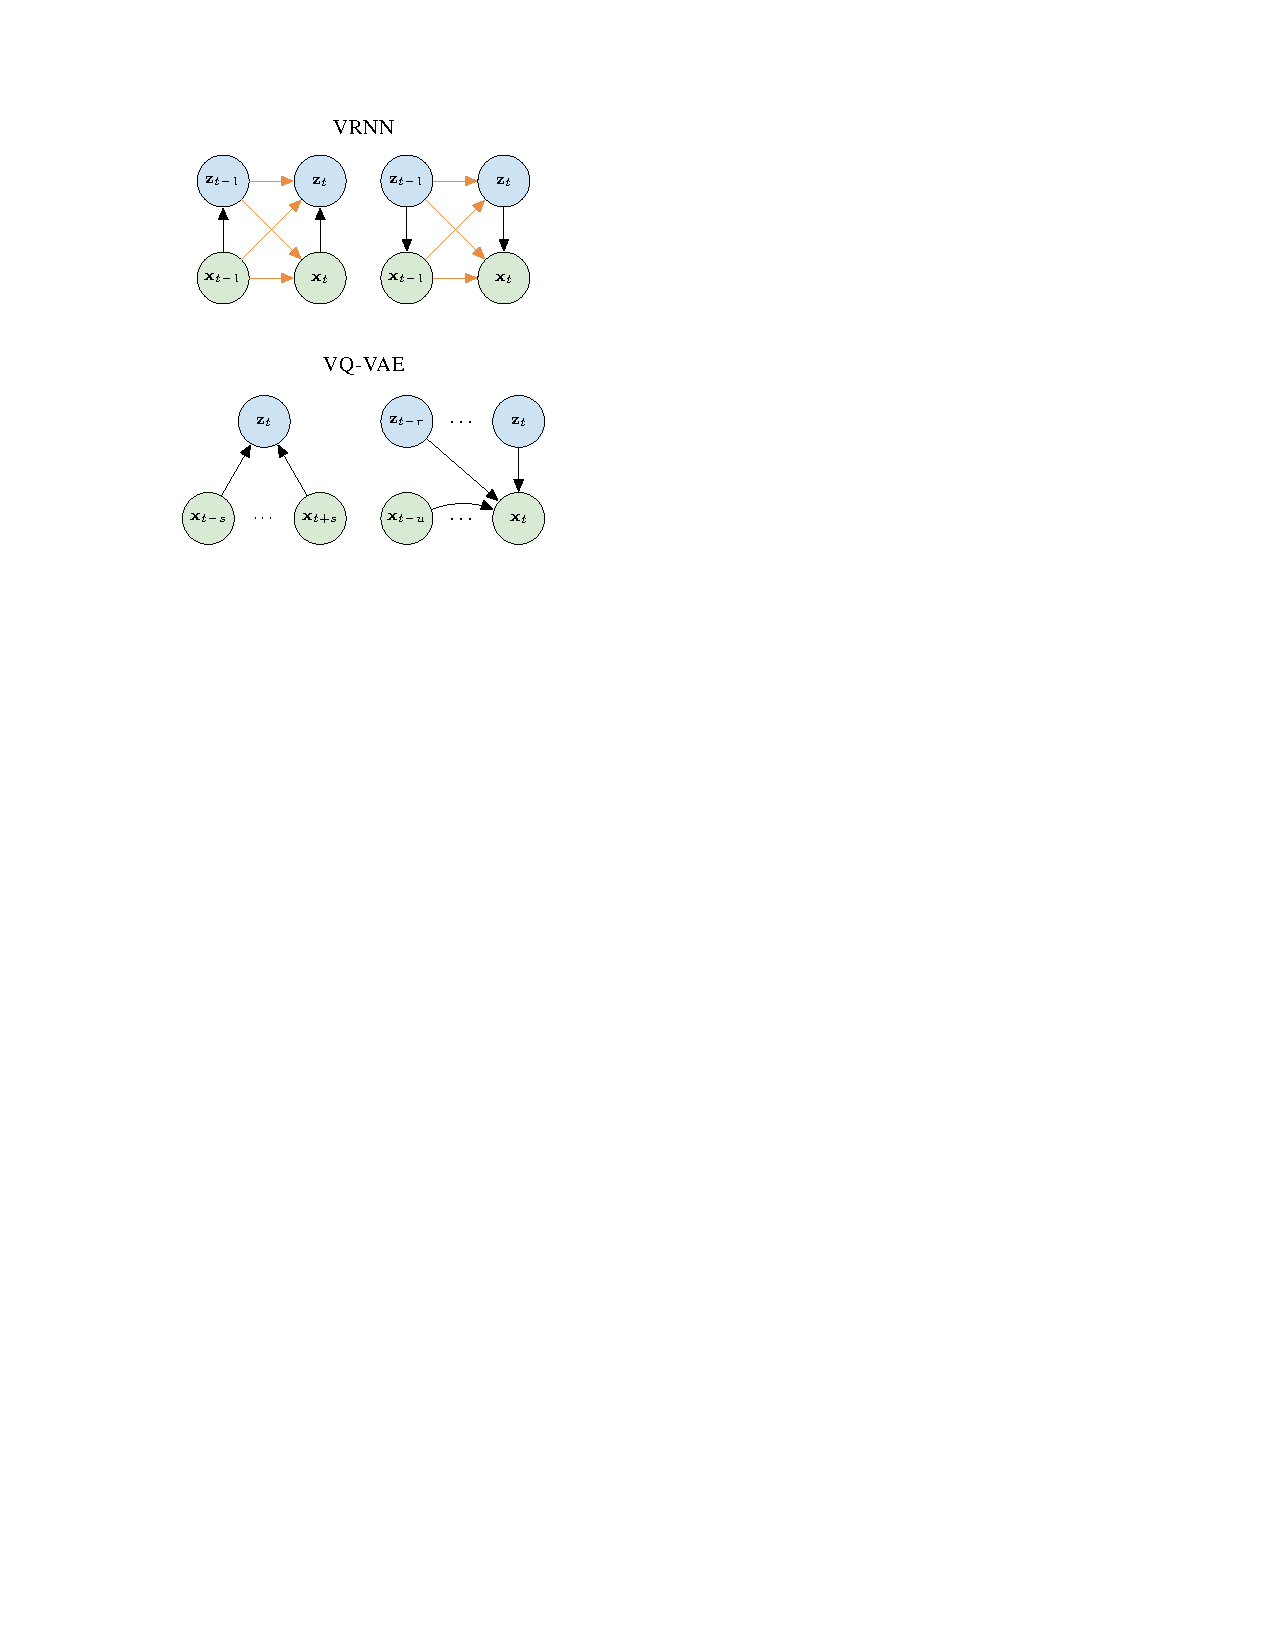
\includegraphics[width=0.8\textwidth]{figures/brief-vrnn-vqvae.pdf}
            \end{figure}
        \end{column}

        \begin{column}{0.5\textwidth}
            \begin{figure}
                \centering
                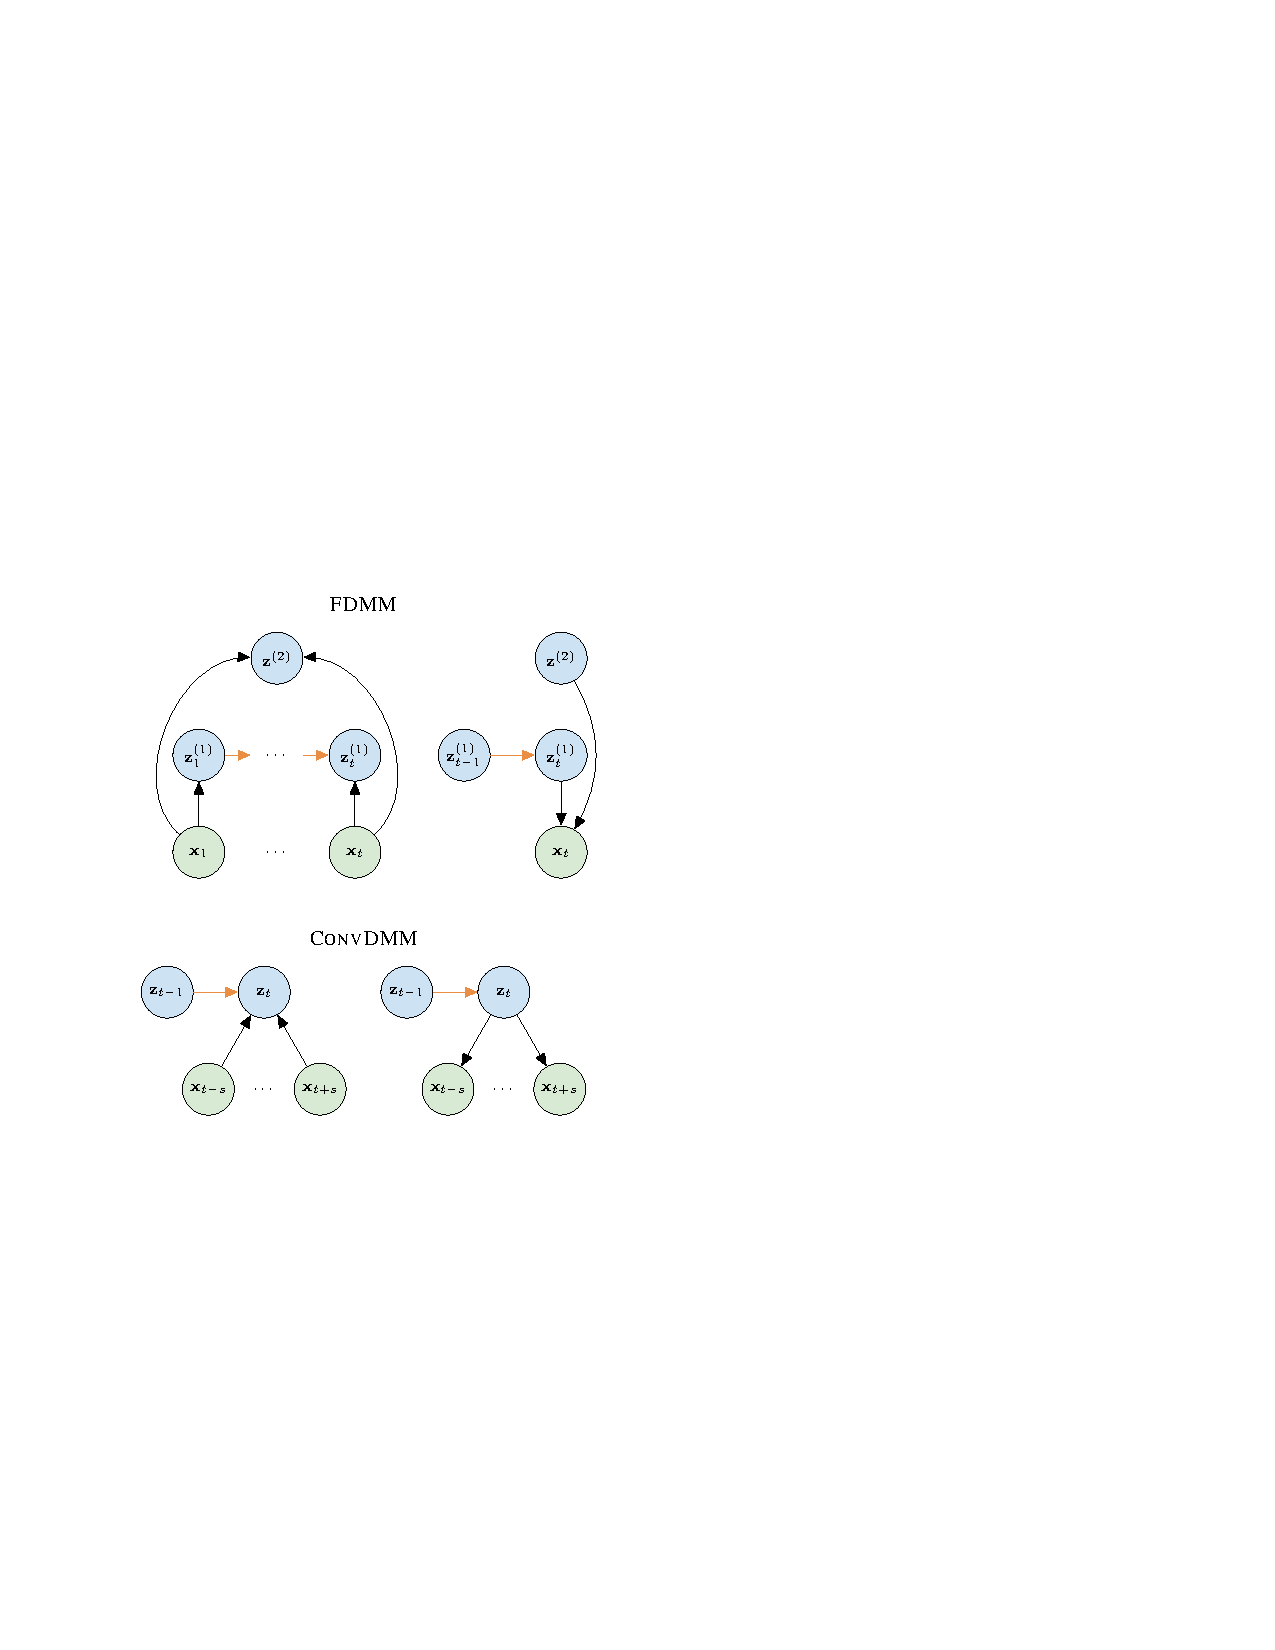
\includegraphics[width=0.8\textwidth]{figures/brief-fdmm-convdmm.pdf}
            \end{figure}            
        \end{column}

    \end{columns}

    \definecolor{sharedcolor}{RGB}{234 142 67} % mørk orange
    \blfootnote{\scalebox{0.6}{{\color{sharedcolor} Orange edges} indicate parameters shared between inference and generative models.}}
\end{frame}


\begin{frame}
    \frametitle{Overview of LVM probabilistic components}

    \begin{table}
        % \caption[A comprehensive overview of observation, prior and inference models for VAE type latent variable models with a single latent variable.]{ A comprehensive overview of observation, prior and inference models for VAE type latent variable models with a single latent variable. The observation, prior and inference models may all belong to one or more of the categories listed under them as detailed in \cref{sec:plvms}. The types listed here serve as primitives from which more complex structures can be constructed including models with hierarchies of multiple latent variables.}
        % \label{tab:lvm-model-primitives}
        % \begin{center}
        \centering
        % \renewcommand{\arraystretch}{1.1}
        \resizebox{0.8\textheight}{!}{%
            \begin{tabular}{ l l l } 
                \toprule
                \multicolumn{2}{l}{\textbf{\textsc{Type}}} & \textbf{\textsc{Form}} \\
                \midrule
                \multicolumn{3}{c}{\textsc{Observation model}} \\
                \midrule
                \textbf{\textsc{arx}} & Autoregressive on $\mathbf{x}_t$      & $p(\mathbf{x}_t|\mathbf{x}_{1:t-1})$ \\
                \textbf{\textsc{loc}} & Local latent variable                 & $p(\mathbf{x}_{t}|\mathbf{z}_{1:t})$ \\
                \textbf{\textsc{glb}} & Global latent variable                & $p(\mathbf{x}_{t}|\mathbf{z})$ \\
                \midrule
                \multicolumn{3}{c}{\textsc{Prior}} \\
                \midrule
                \textbf{\textsc{arx}} & Autoregressive on $\mathbf{x}_t$      & $p(\mathbf{z}_t|\mathbf{x}_{1:t-1})$ \\
                \textbf{\textsc{arz}} & Autoregressive on $\mathbf{z}_t$      & $p(\mathbf{z}_t|\mathbf{z}_{1:t-1})$ \\
                \textbf{\textsc{ind}} & Locally independent $\mathbf{z}_t$                 & $p(\mathbf{z}_t)$ \\
                \textbf{\textsc{glb}} & Global latent variable                & $p(\mathbf{z})$ \\
                \midrule
                \multicolumn{3}{c}{\textsc{Inference model}} \\
                \midrule
                \textbf{\textsc{arz}} & Autoregressive on $\mathbf{z}_t$      & $q(\mathbf{z}_t|\mathbf{z}_{1:t-1})$ \\
                \textbf{\textsc{flt}} & Filtering                             & $q(\mathbf{z}_t|\mathbf{x}_{1:t})$ \\
                \textbf{\textsc{lsm}} & Local smoothing                       & $q(\mathbf{z}_t|\mathbf{x}_{t-r:t+r})$ \\
                \textbf{\textsc{gsm}} & Global smoothing                      & $q(\mathbf{z}_t|\mathbf{x}_{1:T})$ \\
                \textbf{\textsc{glb}} & Global latent variable                & $q(\mathbf{z}|\mathbf{x}_{1:T})$ \\
                \bottomrule
            \end{tabular}
        }
        % \end{center}
    \end{table}

\end{frame}


\begin{frame}
    \frametitle{Classification of selected LVMs for speech}

    \begin{table}
        % \caption[Classification of selected latent variable models.]{ Selected latent variable models classified according the attributes defined throughout \cref{sec:plvms}. See \cref{tab:lvm-model-primitives} for the probability distributions that correspond to each of the attribute short-hands. \textbf{\textsc{hie}} indicates a hierarchical representation.}
        % \label{tab:lvm-taxonomy}
        % \begin{center}
        \centering
        \setlength{\tabcolsep}{3pt}
        \renewcommand{\arraystretch}{1.1}
        \resizebox{0.7\textwidth}{!}{%
            \begin{tabular}{ l | c c c | c c c c | c c c c c | c } 
                \toprule
                \multicolumn{2}{c}{} & 
                \multicolumn{3}{c}{\textsc{Observation}} & 
                \multicolumn{4}{c}{\textsc{Prior}} & 
                \multicolumn{5}{c}{\textsc{Inference}} \\
                \textbf{\textsc{model}} & 
                \textbf{\textsc{arx}} & 
                \textbf{\textsc{loc}} & 
                \textbf{\textsc{glb}} &  
                \textbf{\textsc{arx}} & 
                \textbf{\textsc{arz}} & 
                \textbf{\textsc{ind}} & 
                \textbf{\textsc{glb}} &  
                \textbf{\textsc{arz}} & 
                \textbf{\textsc{flt}} & 
                \textbf{\textsc{lsm}} & 
                \textbf{\textsc{gsm}} & 
                \textbf{\textsc{glb}} &
                \textbf{\textsc{hie}} \\
                \midrule
                %                                                              OBSERVATION       |              PRIOR                |                  INFERENCE       
                %                                                         ARX      LOC      GLB      ARX      ARZ     IND      GLB      ARZ      FLT      LSM      GSM      GLB
                \textbf{VRNN} \footnotesize{\parencite{chung_recurrent_2015}}          & \cmark & \cmark & \xmark & \cmark & \cmark & \xmark & \xmark & \cmark & \cmark & \xmark & \xmark & \xmark & \xmark \\
                \textbf{SRNN} \footnotesize{\parencite{fraccaro_sequential_2016}}      & \cmark & \cmark & \xmark & \cmark & \cmark & \xmark & \xmark & \cmark & \xmark & \xmark & \cmark & \xmark & \xmark \\
                \textbf{HMM-VAE} \footnotesize{\parencite{ebbers_hidden_2017}}         & \xmark & \cmark & \xmark & \xmark & \cmark & \xmark & \xmark & \cmark & \cmark & \xmark & \xmark & \xmark & \cmark \\
                \textbf{ConvVAE} \footnotesize{\parencite{hsu_learning_2017}}          & \xmark & \xmark & \cmark & \xmark & \xmark & \xmark & \cmark & \xmark & \xmark & \xmark & \cmark & \cmark & \xmark \\
                \textbf{FHVAE} \footnotesize{\parencite{hsu_unsupervised_2017}}        & \xmark & \cmark & \cmark & \xmark & \xmark & \cmark & \cmark & \xmark & \xmark & \xmark & \cmark & \cmark & \cmark \\
                \textbf{VQ-VAE} \footnotesize{\parencite{oord_neural_2018}}            & \cmark & \cmark & \xmark & \xmark & \xmark & \cmark & \xmark & \xmark & \xmark & \cmark & \xmark & \xmark & \xmark \\
                \textbf{BHMM-VAE} \footnotesize{\parencite{glarner_full_2018}}         & \xmark & \cmark & \xmark & \xmark & \cmark & \xmark & \xmark & \cmark & \cmark & \xmark & \xmark & \xmark & \xmark \\
                \textbf{STCN} \footnotesize{\parencite{aksan_stcn_2019}}               & \xmark & \cmark & \xmark & \cmark & \xmark & \xmark & \xmark & \xmark & \cmark & \xmark & \xmark & \xmark & \cmark \\
                \textbf{FDMM} \footnotesize{\parencite{khurana_factorial_2019}}        & \xmark & \cmark & \cmark & \xmark & \cmark & \xmark & \cmark & \cmark & \cmark & \xmark & \xmark & \cmark & \cmark \\
                \textbf{ConvDMM} \footnotesize{\parencite{khurana_convolutional_2020}} & \xmark & \cmark & \xmark & \xmark & \cmark & \xmark & \xmark & \cmark & \xmark & \cmark & \xmark & \xmark & \xmark \\
                \bottomrule
            \end{tabular}
        }
        % \end{center}
    \end{table}

\end{frame}

\begin{frame}
    \frametitle{Comparison of LVMs and SSL methods}

    \begin{table}
        % \caption[Classification of selected self"=supervised and probabilistic latent variable models.]{ Selected models classified according to the binary attributes identified throughout the text. The models are sorted according to first publication date on arXiv which might differ from the citation year. \textbf{\textsc{msk}}: masking, \textbf{\textsc{prd}}: prediction, \textbf{\textsc{con}}: contrastive, \textbf{\textsc{rec}}: reconstruction, \textbf{\textsc{qtz}}: quantization, \textbf{\textsc{gen}}: generative, \textbf{\textsc{frz}}: frozen, \textbf{\textsc{ftn}}: fine"=tuned, \textbf{\textsc{loc}}: local, \textbf{\textsc{glo}}: global.}
        % \label{tab:model-taxonomy}
        % \begin{center}
        \centering
        \setlength{\tabcolsep}{3pt}
        \renewcommand{\arraystretch}{1.1}
        \resizebox{1\textheight}{!}{%
            \begin{tabular}{ l l | c c c c c c | c c c | c c } 
                \toprule
                
                \multicolumn{2}{c}{} & 
                \multicolumn{6}{c}{\textsc{model and task design}} & 
                \multicolumn{3}{c}{\textsc{resolution}} &
                \multicolumn{2}{c}{\makebox[0pt][c]{\textsc{usage}}} \\
                & \textbf{\textsc{model}} &
                \textbf{\textsc{msk}} & 
                \textbf{\textsc{prd}} & 
                \textbf{\textsc{con}} &  
                \textbf{\textsc{rec}} &  
                \textbf{\textsc{qtz}} & 
                \textbf{\textsc{gen}} & 
                \textbf{\textsc{loc}} & 
                \textbf{\textsc{glb}} & 
                \textbf{\textsc{var}} & 
                \textbf{\textsc{frz}} & 
                \textbf{\textsc{ftn}} \\
                
                \midrule
                % \multicolumn{11}{c}{\textsc{Self-supervised models}} \\
                % \midrule
                %                                                           MSK      PRD      CON      REC      QTZ      GEN      LOC      GLB     VAR      FRZ      FTN
                \verticalmultirow{9}{\textsc{Self-supervised models}} 
                % & \textbf{Audio Word2vec} \footnotesize{\parencite{chung_audio_2016}}      & \cmark & \xmark & \xmark & \cmark & \xmark & \xmark & \xmark & \cmark & \xmark & \cmark & \xmark \\
                % & \textbf{Speech2Vec} \footnotesize{\parencite{chung_speech2vec_2018}}     & \xmark & \cmark & \xmark & \cmark & \xmark & \xmark & \xmark & \cmark & \xmark & \cmark & \xmark \\
                % & \textbf{Unspeech} \footnotesize{\parencite{milde_unspeech_2018}}         & \xmark & \cmark & \cmark & \xmark & \xmark & \xmark & \xmark & \cmark & \xmark & \cmark & \xmark \\
                
                & \textbf{CPC} \footnotesize{\parencite{oord_representation_2018}}         & \xmark & \cmark & \cmark & \xmark & \xmark & \xmark & \cmark & \xmark & \xmark & \cmark & \xmark \\
                
                & \textbf{APC} \footnotesize{\parencite{chung_unsupervised_2019}}          & \xmark & \cmark & \xmark & \cmark & \xmark & \xmark & \cmark & \xmark & \xmark & \cmark & \xmark \\ % 5/4
                & \textbf{wav2vec} \footnotesize{\parencite{schneider_wav2vec_2019}}       & \xmark & \cmark & \cmark & \xmark & \xmark & \xmark & \cmark & \xmark & \xmark & \cmark & \xmark \\ % 11/4
                & \textbf{Mockingjay}  \footnotesize{\parencite{liu_mockingjay_2020}}      & \cmark & \xmark & \xmark & \cmark & \xmark & \xmark & \cmark & \xmark & \xmark & \cmark & \cmark \\ % 25/10-19
                & \textbf{wav2vec 2.0} \footnotesize{\parencite{baevski_wav2vec_2020}}     & \cmark & \xmark & \cmark & \xmark & \cmark & \xmark & \cmark & \xmark & \xmark & \xmark & \cmark \\ % 20/6
                & \textbf{NPC} \footnotesize{\parencite{liu_nonautoregressive_2020}}       & \cmark & \xmark & \xmark & \cmark & \cmark & \xmark & \cmark & \xmark & \xmark & \cmark & \xmark \\ % 1/11
                & \textbf{DeCoAR 2.0} \footnotesize{\parencite{ling_decoar_2020}}          & \cmark & \xmark & \xmark & \cmark & \cmark & \xmark & \cmark & \xmark & \xmark & \cmark & \xmark \\ % 11/12
                % & \textbf{SCPC} \footnotesize{\parencite{bhati_segmental_2021}}            & \xmark & \cmark & \cmark & \xmark & \xmark & \xmark & \cmark & \xmark & \cmark & \cmark & \xmark \\ % 3/6
                & \textbf{HuBERT} \footnotesize{\parencite{hsu_hubert_2021}}               & \cmark & \xmark & \xmark & \xmark & \cmark & \xmark & \cmark & \xmark & \xmark & \xmark & \cmark \\ % 14/6
                & \textbf{data2vec} \footnotesize{\parencite{baevski_data2vec_2022}}       & \cmark & \xmark & \xmark & \xmark & \xmark & \xmark & \cmark & \xmark & \xmark & \xmark & \cmark \\ % 16/6

                \midrule
                % \multicolumn{11}{c}{\textsc{Probabilistic latent variable models}} \\
                % \midrule
                %                                                           MSK      PRD      CON      REC      QTZ      GEN      LOC      GLO     VAR      FRZ      FTN
                \verticalmultirow{8}{\textsc{Latent variable models}}
                & \textbf{VRNN} \footnotesize{\parencite{chung_recurrent_2015}}          & \xmark & \xmark & \xmark & \cmark & \xmark & \cmark & \cmark & \xmark & \xmark & \cmark & \xmark \\
                & \textbf{SRNN} \footnotesize{\parencite{fraccaro_sequential_2016}}      &\xmark & \xmark & \xmark & \cmark & \xmark & \cmark & \cmark & \xmark & \xmark & \cmark & \xmark \\
                % & \textbf{HMM-VAE} \footnotesize{\parencite{ebbers_hidden_2017}}         & \xmark & \xmark & \xmark & \cmark & \xmark & \cmark & \cmark & \xmark & \xmark & \cmark & \xmark \\
                & \textbf{ConvVAE} \footnotesize{\parencite{hsu_learning_2017}}          & \xmark & \xmark & \xmark & \cmark & \xmark & \cmark & \xmark & \cmark & \xmark & \cmark & \xmark \\
                & \textbf{FHVAE} \footnotesize{\parencite{hsu_unsupervised_2017}}        & \xmark & \xmark & \xmark & \cmark & \xmark & \cmark & \cmark & \cmark & \xmark & \cmark & \xmark \\
                & \textbf{VQ-VAE} \footnotesize{\parencite{oord_neural_2018}}            & \xmark & \xmark & \xmark & \cmark & \cmark & \cmark & \cmark & \xmark & \xmark & \cmark & \xmark \\
                % & \textbf{BHMM-VAE} \footnotesize{\parencite{glarner_full_2018}}         & \xmark & \xmark & \xmark & \cmark & \xmark & \cmark & \cmark & \xmark & \xmark & \cmark & \xmark \\
                & \textbf{STCN} \footnotesize{\parencite{aksan_stcn_2019}}               & \xmark & \xmark & \xmark & \cmark & \xmark & \cmark & \cmark & \xmark & \xmark & \cmark & \xmark \\
                & \textbf{FDMM} \footnotesize{\parencite{khurana_factorial_2019}}        & \xmark & \xmark & \xmark & \cmark & \xmark & \cmark & \cmark & \cmark & \xmark & \cmark & \xmark \\
                & \textbf{ConvDMM} \footnotesize{\parencite{khurana_convolutional_2020}} & \xmark & \xmark & \xmark & \cmark & \xmark & \cmark & \cmark & \xmark & \xmark & \cmark & \xmark \\
                \bottomrule
            \end{tabular}
        }
        % \end{center}
    \end{table}

\end{frame}


\begin{frame}
    \frametitle{Conclusions}
    \begin{itemize}
        \item {\bfseries Main conclusions}:
        \begin{itemize}
            \item The most popular self-supervised speech models can be compactly described by a few core design choices.
            \item Many of these design choices are mirrored in earlier work on speech embedding models.
        \end{itemize}
        \item {\bfseries Open questions and limitations}:
        \begin{itemize}
            \item Which design choices benefit which downstream tasks?
            \item It is difficult to compare methods as model size and evaluation procedures differ widely between papers.
        \end{itemize}
    \end{itemize}
\end{frame}
